\documentclass[11pt]{article}
\usepackage[utf8]{inputenc}
\usepackage[T1]{fontenc}
\usepackage{geometry}
\usepackage{graphicx}
\usepackage{xcolor}
\usepackage{tikz}
\usetikzlibrary{positioning, arrows.meta}
\usepackage{hyperref}
\hypersetup{colorlinks=true, linkcolor=blue, citecolor=blue, urlcolor=blue}

% Adjust margins for readability on A4/Letter paper
\geometry{
  margin=1in,
  headheight=14pt,
  headsep=0.2in
}

\title{Agile \& Scrum Development and KPI Programming for the Workout Planner}
\author{}
\date{\today}

\begin{document}

\maketitle

\section{Introduction}

This document provides an overview of how agile and Scrum methodologies guided the development of the \emph{Workout Planner} web application and how key performance indicators (KPIs) were incorporated both into the development process and the application itself.  The Workout Planner is a React-based tool that allows users to define custom workouts and assign them to different days of the week.  It also computes simple metrics about the plan, mirroring the idea of tracking KPIs in software projects.

\section{Agile Methodology}

Agile software development emphasises short feedback cycles, collaboration and adaptation over rigid processes.  Within the agile family there are many frameworks; however, they share common values such as delivering value quickly, embracing change and empowering teams.

Agile teams often track quantitative measures to evaluate progress.  Atlassian highlights that metrics such as \emph{sprint burndown}, \emph{velocity}, \emph{cycle time} and \emph{cumulative flow diagrams} help teams track progress, identify bottlenecks and forecast future work\footnote{Agile metrics like sprint burndown, velocity, cycle time and cumulative flow diagrams help teams track progress and optimise delivery【885271492900025†L1629-L1634】.}.  Choosing the right metrics and reviewing them regularly enables data–driven decisions and continuous improvement.

A specific metric used to measure success against defined goals is known as a \emph{key performance indicator} (KPI).  In an agile context, KPIs might include customer satisfaction, defect rates or time to market; selecting the right KPIs ensures the team remains focused on delivering value\footnote{A KPI in Agile is a specific metric used to measure the success of a team or project against defined goals; examples include customer satisfaction, defect rates and time to market【885271492900025†L1656-L1672】.}.

\section{Scrum Framework}

\subsection{Overview}

Scrum is an agile framework that structures work into fixed–length \emph{sprints} and encourages iterative delivery.  The Scrum Guide describes Scrum as a \emph{lightweight framework} that helps people, teams and organisations generate value through adaptive solutions for complex problems\footnote{Scrum is a lightweight framework that helps teams generate value through adaptive solutions for complex problems【142831186830001†L69-L71】.}.  It emphasises empiricism—transparency, inspection and adaptation—and lean thinking.  Knowledge emerges from experience; therefore teams regularly inspect their work and processes and adapt accordingly.

\subsection{Roles}

A Scrum Team is a small, cross–functional and self–managing unit composed of one \emph{Product Owner}, one \emph{Scrum Master} and \emph{Developers}.  There are no sub–teams or hierarchies; the team is collectively responsible for delivering a valuable increment every sprint\footnote{The Scrum Team consists of one Scrum Master, one Product Owner and Developers; it is cross–functional and self–managing【142831186830001†L165-L177】.}.  

\begin{itemize}
  \item \textbf{Product Owner}: responsible for maximising product value and managing the Product Backlog\footnote{The Product Owner is accountable for maximising the value of the product and for effective backlog management【142831186830001†L210-L225】.}.
  \item \textbf{Scrum Master}: ensures that Scrum is understood and enacted, coaches the team and removes impediments\footnote{The Scrum Master is accountable for establishing Scrum, coaching the team and removing impediments【142831186830001†L238-L260】.}.
  \item \textbf{Developers}: professionals who create a usable increment each sprint, plan the sprint backlog and adhere to a Definition of Done\footnote{Developers plan the sprint backlog, instil quality by adhering to the Definition of Done and adapt their plan daily【142831186830001†L194-L208】.}.
\end{itemize}

\subsection{Events}

Scrum prescribes five formal events.  Each event is a timeboxed opportunity to inspect and adapt, enabling transparency and regular cadence.  The Sprint is the container for all other events and typically lasts a month or less【142831186830001†L286-L306】.  Within each Sprint:

\begin{itemize}
  \item \textbf{Sprint Planning} sets the goal and selects the work for the sprint.
  \item \textbf{Daily Scrum} is a 15–minute meeting where Developers inspect progress toward the Sprint Goal and adapt the plan【142831186830001†L377-L389】.
  \item \textbf{Sprint Review} involves presenting the increment to stakeholders and discussing what to do next【142831186830001†L400-L410】.
  \item \textbf{Sprint Retrospective} examines how the Sprint went and identifies improvements【142831186830001†L417-L428】.
\end{itemize}

\subsection{Workflow Diagram}

Figure~\ref{fig:scrum-cycle} visualises the Scrum sprint cycle.  The Product Backlog is refined in Sprint Planning; the team executes the Sprint and holds Daily Scrums; at the end of the Sprint, a Sprint Review and Sprint Retrospective inform the next iteration.

\begin{figure}[h]
  \centering
  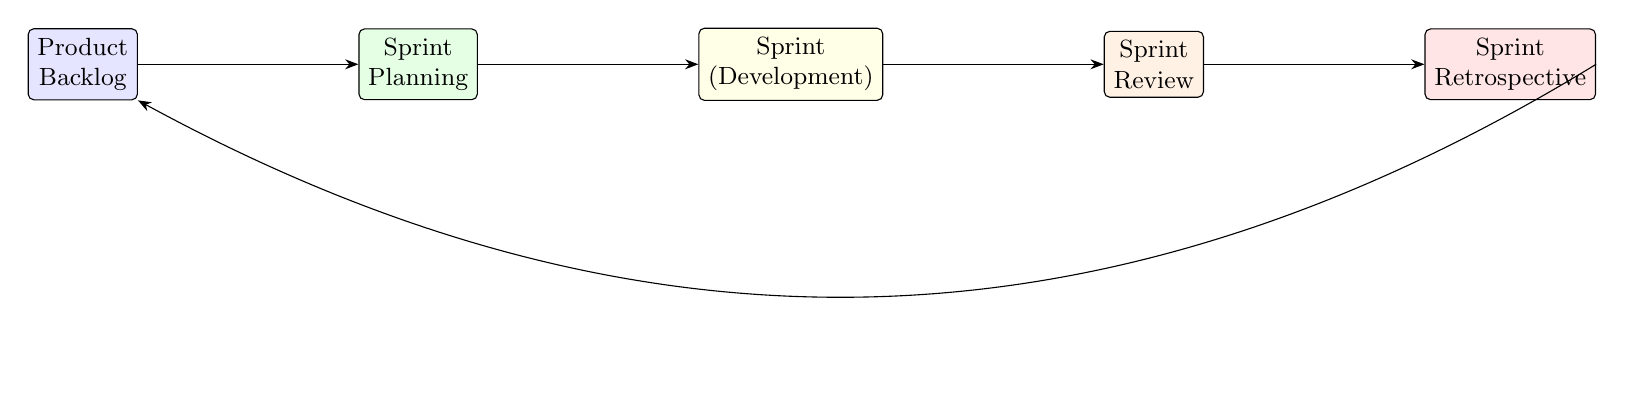
\begin{tikzpicture}[node distance=2.8cm, every node/.style={align=center, font=\small}, >=Stealth]
    \node[rectangle, draw, rounded corners=2pt, fill=blue!10] (backlog) {Product\\Backlog};
    \node[rectangle, draw, rounded corners=2pt, fill=green!10, right=of backlog] (planning) {Sprint\\Planning};
    \node[rectangle, draw, rounded corners=2pt, fill=yellow!10, right=of planning] (sprint) {Sprint\\(Development)};
    \node[rectangle, draw, rounded corners=2pt, fill=orange!10, right=of sprint] (review) {Sprint\\Review};
    \node[rectangle, draw, rounded corners=2pt, fill=red!10, right=of review] (retro) {Sprint\\Retrospective};
    \draw[->] (backlog) -- (planning);
    \draw[->] (planning) -- (sprint);
    \draw[->] (sprint) -- (review);
    \draw[->] (review) -- (retro);
    \draw[->, bend left=30] (retro.east) to (backlog.south east);
  \end{tikzpicture}
  \caption{Scrum sprint cycle highlighting the iterative flow from backlog to planning, development, review and retrospective before starting the next cycle.}
  \label{fig:scrum-cycle}
\end{figure}

\section{Key Performance Indicators (KPIs) in Software Development}

In software projects it is important to measure performance to understand whether the team is delivering value and to identify opportunities for improvement.  Agile teams commonly track a variety of KPIs:

\begin{itemize}
  \item \textbf{Velocity}: the average amount of work a team completes during a sprint, usually measured in story points or hours【885271492900025†L1760-L1777】.  Tracking velocity over multiple sprints helps forecast how quickly a backlog can be delivered.
  \item \textbf{Cycle time and lead time}: the time taken to complete a task or deliver a feature.  These metrics highlight delays and process efficiency.
  \item \textbf{Sprint burndown}: a chart showing the remaining work during a sprint.  Teams use it to visualise progress and ensure they are on track to meet the Sprint Goal【885271492900025†L1695-L1701】.
  \item \textbf{Cumulative flow diagram}: a stacked area chart showing the state of work items over time.  Smooth bands indicate balanced flow, while bubbles suggest bottlenecks.
  \item \textbf{Quality metrics}: escaped defects, defect density, and test coverage help assess the quality of the increment【885271492900025†L1859-L1874】.
\end{itemize}

Selecting KPIs depends on the team’s goals.  When used appropriately they provide actionable insights, but they should never be weaponised; metrics exist to guide improvement rather than to punish teams.

\section{Application to the Workout Planner}

Although the Workout Planner is a small project, applying agile thinking and KPIs enhances its quality and sustainability.  During development the features were broken down into a backlog of tasks, implemented in short iterations, and reviewed to gather feedback.  The project uses Git for version control and a clean repository structure to support collaboration and deployment.

Within the application itself we implemented simple KPIs to mirror the concept of measuring progress.  The planner computes:

\begin{itemize}
  \item \textbf{Total defined exercises}: the number of workouts stored in the catalogue.
  \item \textbf{Total workouts assigned}: the total number of times workouts are scheduled across the week.
  \item \textbf{Average workouts per day}: the mean number of workouts scheduled per day.
  \item \textbf{Workouts per day}: a breakdown of how many workouts are assigned each day.
\end{itemize}

These indicators help users understand whether their training plan is balanced.  For example, scheduling too many workouts on one day may indicate an unrealistic plan, while days with no workouts could present opportunities for active recovery.  Figure~\ref{fig:kpi-example} shows an example KPI chart using sample data.

\begin{figure}[h]
  \centering
  \includegraphics[width=0.7\textwidth]{kpi_example.png}
  \caption{Example KPI chart illustrating the number of workouts per day.  Balanced training plans distribute workload evenly throughout the week.}
  \label{fig:kpi-example}
\end{figure}

\section{Conclusion}

The Workout Planner project illustrates how agile and Scrum methodologies can guide even small software projects.  By organising work into a backlog, iterating through sprints and reviewing progress regularly, the team can adapt quickly and deliver value incrementally.  Incorporating KPIs—both in the development process and within the application itself—provides objective feedback and promotes continuous improvement.  

As the project grows, additional metrics such as defect rate, deployment frequency or user engagement could be added to better understand its impact and drive decisions.  Ultimately, agility and thoughtful measurement enable teams to build better software and provide users with more reliable tools.

\end{document}